\documentclass[12pt,aspectratio=169]{beamer}

\usetheme{metropolis}

\usefonttheme{professionalfonts}
\usepackage{graphicx}
\usepackage{tikz}
\usepackage{amsmath}
\usepackage{mathpazo}
\usepackage{xcolor,colortbl}
\usepackage{siunitx}
\usepackage[siunitx]{circuitikz} % to draw circuits!

\setmonofont{Ubuntu Mono}
\setlength{\parskip}{0pt}
\renewcommand{\baselinestretch}{1}

\sisetup{
  number-math-rm=\mathnormal,
  per-mode=symbol
}

\title{Magnetism}
\subtitle{Special CAP/AP Lecture}
\author[TML]{Dr.\ Timothy Leung}
\institute{Olympiads School, Toronto, ON, Canada}
\date{November 2019}


\newcommand{\pic}[2]{\includegraphics[width=#1\textwidth]{#2}}
\newcommand{\mb}[1]{\mathbf{#1}}
\newcommand{\eq}[2]{\vspace{#1}{\Large\begin{displaymath}#2\end{displaymath}}}

\begin{document}

\begin{frame}
  \maketitle
\end{frame}


%\section[Intro]{Introduction}
%
%\begin{frame}
%  \frametitle{Files for You to Download}
%  Download from the school website:
%  \begin{enumerate}
%  \item\texttt{12-Magnetism.pdf}---This presentation. If you want to print the
%    slides on paper, I recommend printing 4 slides per page.
%  \item\texttt{12-Homework.pdf}---Homework assignment for Topics 11 and 12.
%  \end{enumerate}
%
%  \vspace{.2in}Please download/print the PDF file before each class. When you
%  are taking notes, pay particular attention to things I say that aren't
%  necessarily on the slides.
%\end{frame}



\section{Magnetic Field}

\begin{frame}{Review of Magnetic Field}{Remember Physics 12?}
  \begin{itemize}
  \item Magnetism is generated by moving charged particles, e.g.
    a single charge, or an electric current
  \item It can also be generated by permanent magnets, or Earth
  \end{itemize}
\end{frame}



\begin{frame}{Review of Magnetic Field}
  \begin{itemize}
  \item Magnetism affects other \emph{moving} charged particles
  \item The vector field is called the \textbf{magnetic field}
  \item Magnetic field has unit \textbf{tesla}
  \item Magnetic field lines have no ends---they always run in a loop
  \end{itemize}
\end{frame}



\begin{frame}{Magnetic Field Generated by a Moving Point Charge}
  \begin{center}
    \pic{.35}{pointchargeB.png}
  \end{center}
  A point charge generates an electric field $\mb{E}$. When it's moving, it
  also generates a magnetic field $\mb{B}$, given by the equation:

  \eq{-.2in}{
    \boxed{\mb{B}=\frac{\mu_0}{4\pi}\frac{q\mb{v}\times\hat{\mb{r}}}{r^2}}
  }

  The direction of $\mb{B}$ can be obtained by applying the
  \emph{right hand rule} if you are not confident with cross products.
\end{frame}



%\begin{frame}{Reminder on the cross product}
%  Whenever the ``right hand rule'' is mentioned, or when an equation has
%  ``$\sin\theta$'' in it, that usually means that the equation involces a
%  cross product in it. Just a reminder on a few properties:
%  \begin{itemize}
%  \item If $\mb{C}=\mb{A}\times\mb{B}$, then $\mb{C}$ is perpendicular to both
%    $\mb{A}$ and $\mb{B}$.
%  \item The length of the cross product of two vectors is:
%    
%    \eq{-.3in}{
%      |\mb{A}\times\mb{B}|=|\mb{A}||\mb{B}|\sin\theta
%    }
%    where $\theta$ is the angle between $\mb{A}$ and $\mb{B}$
%  \item Cross products are anti-commutable:
%
%    \eq{-.35in}{
%      \mb{A}\times\mb{B}=-\mb{B}\times\mb{A}
%    }
%  \end{itemize}
%\end{frame}



\begin{frame}{Magnetic Field Generated by a Moving Point Charge}

  \eq{-.05in}{
    \boxed{\mb{B}=\frac{\mu_0}{4\pi}\frac{q\mb{v}\times\hat{\mb{r}}}{r^2}}
  }
  \begin{center}
    \begin{tabular}{l|c|l}
      \rowcolor{pink}
      \textbf{Quantity} & \textbf{Symbol} & \textbf{SI Unit} \\ \hline
      Magnetic field                  & $\mb{B}$ & \si{\tesla}\\
      Charge                          & $q$      & \si{\coulomb}\\
      Velocity of the charge          & $\mb{v}$ & \si{m/\second}\\
      Distance from the moving charge & $r$      & \si{\metre}\\
      Radial outward unit vector from the charge & $\hat{\mb{r}}$ & no units\\
      Permeability of free space & $\mu_0$ & \si{\tesla.\metre\per\ampere}
    \end{tabular}
  \end{center}
  \textbf{Permeability of free space} (or \textbf{vacuum permeability}) is a
  constant with a value of $\mu_0=\SI{4\pi e-7}{\tesla.\metre\per\ampere}$. It
  is a measure of how well a space can become magnetized.
\end{frame}



\begin{frame}{Magnetic Generated By a Current}{Biot-Savart Law}
  \begin{columns}
    \column{.25\textwidth}
    \pic{1}{bsav.png}
    
    \column{.75\textwidth}
    An electric current is really many charges particles moving along a wire;
    each charge creating its own magnetic field.
    The total magnetic field in the wire is the integral of the contribution
    ($d\mb{B}$) of the current ($I$) from each infinitesimal sections
    ($d\mb{L}$) of the wire, given by the \textbf{Biot-Savart law}:
  
    \eq{-.2in}{
      \boxed{d\mb{B}=\frac{\mu_0}{4\pi}\frac{Id\mb{L}\times\hat{\mb{r}}}{r^2}}
    }

    The magnetic field in the diagram goes \emph{into} the page
  \end{columns}
\end{frame}


\begin{frame}{Magnetic Field Generated By an Infinitely Long Wire}
  \begin{columns}
    \column{.2\textwidth}
    \pic{1}{magcur2.png}
    
    \column{.7\textwidth}
    Integrating Biot-Savart law for a point at radial distance $r$ from an
    \emph{infinitely long wire} gives a simple expression:

    \eq{-.35in}{
      \boxed{\mb{B}=\frac{\mu_0(\mb{I}\times\mb{\hat{r})}}{2\pi r}}
      \quad\text{or}\quad
      \boxed{B=\frac{\mu_0I}{2\pi r}}
    }

    \vspace{-.15in}The magnitude and direction current ``vector'' $\mb{I}$ is
    straightforward
    
    \vspace{.1in}\begin{tabular}{l|c|c}
      \rowcolor{pink}
      \textbf{Quantity} & \textbf{Symbol} & \textbf{SI Unit} \\ \hline
      Magnetic field      & $\mb{B}$ & \si{\tesla} \\
      Current             & $\mb{I}$ & \si{\ampere} \\
      Radial direction from the wire & $\mb{\hat{r}}$ & (no units)\\
      Radial distance from the wire  & $r$            & \si{\metre}
    \end{tabular}
  \end{columns}
\end{frame}


\begin{frame}{Current-Carrying Wire Loop}
  \begin{columns}
    \column{.35\textwidth}
    \pic{1}{curloo.png}

    \column{.65\textwidth}
    When we shape the current-carrying wire into a loop, we can (again) use
    the Biot-Savart law to find the magnetic field away from it.

    \vspace{.2in}
    One loop isn't very interesting (except when you're integrating Biot-Savart
    law) but what if we have many loops
  \end{columns}
\end{frame}



\begin{frame}{Wounding Wires Into a Coil}
  \begin{itemize}
  \item A \textbf{solenoid} is when you wound a wire into a coil
  \item You create a magnet very similar to a bar magnet, with an effective
    north pole and a south pole
  \item Magnetic field inside the solenoid is uniform
  \item Magnetic field strength can be increased by the addition of an iron core
  \end{itemize}
  \begin{center}
    \pic{.5}{barsol.png}
  \end{center}
\end{frame}



\begin{frame}{A Practical Solenoid}
  A practical solenoid usually has hundreds or thousands of turns:
  \begin{center}
    \pic{.45}{1020201515330450255.jpg}
  \end{center}

  \vspace{-.2in}
  This ``air core'' coil is used for high school and university experiments. It
  has approximately 600 turns of copper wire wound around a plastic core.
\end{frame}

\begin{frame}{Magnetic Field Inside a Solenoid}
  \begin{columns}
    \column{.3\textwidth}
    \pic{1.1}{magneticfield4.png}
    \column{.7\textwidth}
    The magnetic field \textbf{inside} a solenoid is uniform, with its strength
    given by:
    
    \eq{-.2in}{
      \boxed{B=\frac{\mu NI}{L}}
    }
    
    Direction of $\mb{B}$ determined by \textbf{right hand rule}

    \vspace{.1in}\begin{tabular}{l|c|c}
      \rowcolor{pink}
      \textbf{Quantity} & \textbf{Symbol} & \textbf{SI Unit} \\ \hline
      Magnetic field intensity & $B$ & \si{\tesla} \\
      Number of coils          & $N$ & \\
      Lenght of the solenoid   & $L$ & \si{\metre}\\
      Current                  & $I$ & \si{\ampere}\\
      Effective permeability & $\mu$ & \si{T.m/A}
    \end{tabular}
  \end{columns}
\end{frame}



\section{Amp\`{e}re's Law}

\begin{frame}{Amp\`{e}re's Law}
  \begin{columns}
    \column{.25\textwidth}
    \pic{1}{amlaw.png}
    
    \column{.75\textwidth}
    Like Gauss's law is used to calculate electric fields,
    \textbf{Amp\`{e}re's law} is used to calculate the magnetic field for
    symmetric configurations:

    \eq{-.1in}{\boxed{\oint_C \mb{B}\cdot d\boldsymbol{\ell}=\mu_0 I_C}}
    where
    \begin{itemize}
    \item $C$ is a closed curve around a current (``Amperian loop'')
    \item $d\boldsymbol{\ell}$ is an infinitesimal length along the closed curve
    \item $I_c$ is the net current that penetrates the area bounded by $C$
    \end{itemize}
  \end{columns}
\end{frame}



\begin{frame}{Application of Amp\`{e}re's Law: Infinitely Long Wire}
  \begin{columns}
    \column{.3\textwidth}
    \pic{1}{4iM3O.png}

    \column{.7\textwidth}
    An \emph{infinitely} long wire must generate a magnetic field that only
    depend on radial distance. We place an Amperian loop as a circle of radius
    $r$ inside the toroid. Amp\`{e}re's law reduces to:

    \eq{-.3in}{
      \oint_C \mb{B}\cdot d\boldsymbol{\ell}=\mu_0 I_C
      \;\rightarrow\;
      B(2\pi r)=\mu_0 I
    }
      
    From this, we get our expression of the magnetic field from an infinitely
    long wire:
      
    \eq{-.2in}{
      B=\frac{\mu_0 I}{2\pi r}
    }
  \end{columns}
\end{frame}



\begin{frame}{Toroid}
  \begin{columns}
    \column{.3\textwidth}
    \pic{1.1}{toroid.png}

    {\scriptsize A toroid consists of a current-\\
      carrying wire wound around a donut-shaped core \par}
    
    \column{.7\textwidth}
    Another application of Amp\`{e}re's law is the \textbf{toroid}. This time,
    we put our loop at $a<r<b$ inside the toroid. Once again, because of
    symmetry, Amp\`{e}re's law reduces to:

    \vspace{-.35in}{\Large
      \begin{align*}
        \oint_C \mb{B}\cdot d\boldsymbol{\ell}&=\mu_0 I_C\\
        B(2\pi r)&=\mu_0 NI\\
        B&=\frac{\mu_0 NI}{2\pi r}
      \end{align*}
    }

    \vspace{-.15in}where $N$ is the number of times the wire is wound around
    the core
    
  \end{columns}
\end{frame}


\begin{frame}{Toroid}
  \begin{columns}
    \column{.3\textwidth}
    \pic{1.15}{toroid.png}

    \column{.7\textwidth}
    When the loop is placed at $r<a$, there is no enclosed
    current, and therefore the magnetic field is zero:

    \eq{-.3in}{B=0\quad\text{for}\quad r<a}

    \vspace{-.2in}When the loop is placed at $r>b$, the amount of current
    penetrating the loop is the same in both direction, i.e.\ $I_c=0$, and

    \eq{-.3in}{B=0\quad\text{for}\quad r>b}
    
    \vspace{-.1in}In fact, magnetic field \emph{only} exists inside the core,
    between $a$ and $b$.
%    
%    \eq{-.2in}{
%      B=\frac{\mu_0 NI}{2\pi r}\quad\text{for}\quad a\leq r\leq b
%    }
  \end{columns}
\end{frame}




\section{Magnetic Force}

\begin{frame}{So What Does the Magnetic Field Do?}{In Classical Physics}
  \begin{columns}
    \column[t]{.3\textwidth}
    \begin{center}
      Gravitational Field $\mb{g}$
    \end{center}
    \begin{itemize}
    \item Generated by objects with mass
    \item Affects objects with mass
    \end{itemize}

    \column[t]{.3\textwidth}
    \begin{center}
      Electric Field $\mb{E}$
    \end{center}
    \begin{itemize}
    \item Generated by charged particles
    \item Affects charged particles
    \end{itemize}

    \column[t]{.4\textwidth}
    \begin{center}
      Magnetic Field $\mb{B}$
    \end{center}
    \begin{itemize}
    \item Generated by \emph{moving} charged particles
    \item Affects moving charged particles
    \end{itemize}
  \end{columns}
\end{frame}



\begin{frame}{Lorentz Force Law}
  Since a moving charge or current create both electric and magnetic fields,
  another moving charge is therefore affected by both $\mb{E}$ and $\mb{B}$.
  The total effect is given by the \textbf{Lorentz force law}:

  \eq{-.2in}{
    \boxed{\mb{F}=q(\mb{E}+\mb{v}\times\mb{B})}
  }

  \vspace{-.1in}$\mb{F}_q=q\mb{E}$ is the electrostatic force, and
  $\mb{F}_M=q\mb{v}\times\mb{B}$ is the magnetic force.
  \begin{center}
    \begin{tabular}{l|c|c}
      \rowcolor{pink}
      \textbf{Quantity} & \textbf{Symbol} & \textbf{SI Unit} \\ \hline
      Total force on the moving charge & $\mb{F}$ & \si{\newton} \\
      Charge                 & $q$      & \si{\coulomb} \\
      Velocity of the charge & $\mb{v}$ & \si{\metre\per\second} \\
      Magnetic field         & $\mb{B}$ & \si{\tesla} \\
      Electric field         & $\mb{E}$ & \si{\newton\per\coulomb}
    \end{tabular}
  \end{center}
\end{frame}



\begin{frame}{Force on a Current-Carrying Conductor in a Magnetic Field}
  Likewise, $\mb{B}$ exerts a force on another current-carrying conductor.

  \eq{-.2in}{
    \boxed{F_M=\mb{I}l\times\mb{B}}
  }
  \begin{center}
    \begin{tabular}{l|c|c}
      \rowcolor{pink}
      \textbf{Quantity} & \textbf{Symbol} & \textbf{SI Unit} \\ \hline
      Magnetic force on the conductor   & $\mb{F}_M$ & \si{\newton} \\
      Electric current in the conductor & $\mb{I}$   & \si{\ampere} \\
      Length of the conductor           & $l$        & \si{\metre} \\
      Magnetic field                    & $\mb{B}$   & \si{\tesla}
    \end{tabular}
  \end{center}
\end{frame}



\begin{frame}{Magnetic Force on Two Current-Carrying Wires}
  \begin{columns}
    \column{.26\textwidth}
    \pic{1.08}{wirefor.png}

    \column{.74\textwidth}
    Two parallel current-carrying wires of length $L$ are at a distance $r$
    apart. Magnetic field at wire $2$ from current $I_1$ has constant strength
    along the wire, given by:

    \eq{-.2in}{
      B=\frac{\mu_0I_1}{2\pi r}
    }

    The force of $B$ on $I_2$ is:

    \eq{-.3in}{
      F=I_2LB=\frac{\mu_0I_1I_2L}{2\pi r}
      \;\rightarrow\;
      \boxed{\frac{F}{L}=\frac{\mu_0I_1I_2}{2\pi r}}
    }

    $I_1$ also exerts the same force on $I_2$, pulling the wires towards each
    other. (We should expect this because of Newton's third law of motion.)
  \end{columns}
\end{frame}



\begin{frame}{Circular Motion Caused by a Magnetic Field}
  When a charged particle enters a magnetic field at right angle\ldots
  \begin{itemize}
  \item Magnetic force $\mb{F}_M$ perpendicular to both velocity $\mb{v}$ and
    magnetic field $\mb{B}$.
  \item Results in circular motion
  \end{itemize}
  Centripetal force $\mb{F}_c$ is provided by the magnetic force $\mb{F}_M$.
  Equating the two expressions:

  \eq{-.4in}{
    \frac{mv^2}{r}=qvB
  }
  
  We can solve for $r$ get the radius for a charge with a known
  mass, or solve for mass $m$ of a charged particle based on its radius:  

  \eq{-.2in}{
    r = \frac{mv}{qB}\quad\quad\quad m=\frac{qrB}{v}
  }
\end{frame}



\section{Faraday's Law}

\begin{frame}{Magnetic Flux}
  \textbf{Question:} If a current-carrying wire can generate a magnetic field,
  can a magnetic field affect the current in a wire?

  \vspace{.3in}\textbf{Answer:} Yes, sort of\ldots

  \vspace{.3in}To understand how to \emph{induce} a curent by a magnetic field,
  we need to look at fluxes again.
\end{frame}


\begin{frame}{Magnetic Flux}
  \begin{columns}
    \column{.4\textwidth}
    \pic{1.1}{flux2.png}
  
    \column{.6\textwidth}
    Magnetic flux is defined as:
    
    \eq{-.15in}{
      \boxed{\Phi_M=\int\mb{B}\cdot d\mb{A}}
    }
    
    where $\mb{B}$ is the magnetic field, and $d\mb{A}$ is the infinitesimal
    area pointing \textbf{outwards}. Note that magnetic flux can also be
    expressed as:

    \eq{-.2in}{
      \boxed{\Phi_M=\int\mb{B}\cdot\hat{\mb{n}}dA}
    }

    where $\hat{\mb{n}}$ is the outward normal direction
  \end{columns}
\end{frame}



\begin{frame}{Magnetic Flux Over a Closed Surface}
  The unit for magnetic flux is a ``weber'' (\si{\weber}), in honor of German
  physicist Wilhelm Weber, who invented the electromagnetic telegraph with Carl
  Gauss. The unit is defined as:

  \eq{-.3in}{\SI{1}{\weber}=\SI{1}{\tesla.\metre^2}}
  
  \vspace{-.2in}The magnetic flux over a closed surface is always zero:

  \eq{-.2in}{
    \boxed{\oint\mb{B}\cdot d\mb{A}=0}
  }

  Since magnetic field lines only exist as a loop, that means there should be
  equal amount of ``flux'' flowing out of a closed surface as entering the
  surface.
\end{frame}


%\begin{frame}{Magnetic Flux}
%  \begin{center}
%    \pic{.4}{flux2.png}
%  \end{center}
%
%  
%
%  \vspace{-.15in}Not surprisingly, the magnetic flux is defined similar to
%  electric flux:
%  
%  \eq{-.2in}{
%    \boxed{\Phi_\mathrm{magnetic}=\int\mb{B}\cdot d\mb{A}}
%  }
%
%  where $\mb{B}$ is the magnetic field, and $d\mb{A}$ is the infinitesimal area
%  with its direction point outward.
%\end{frame}
%
%\begin{frame}
%  \frametitle{Magnetic Flux Over a Closed Surface}
%
%  The magnetic flux over a closed surface is always zero:
%
%  \eq{-.2in}{
%    \boxed{\oint\mb{B}\cdot d\mb{A}=0}
%  }
%
%  Since magnetic field exists in a loop only, what every flux that leaves the
%  surface has to eventually come back.
%\end{frame}


\begin{frame}{Changing Magnetic Flux}
  Changes to magnetic flux can be due to a number of reasons:
  \begin{enumerate}
  \item\textbf{Changing magnetic field}\ldots if the magnetic field is created
    by a time-dependent source (e.g.\ alternating current)
  \item\textbf{Changing orientation of magnetic field} either because the
    surface area is moving relative to the magnetic field.
  \item\textbf{Changing area} the surface area from which the flux is
    calculated is changing.
  \end{enumerate}
\end{frame}


\begin{frame}{When Magnetic Flux is Changing}
  \begin{itemize}
  \item When the magnetic flux $\Phi_M$ is changing, an electromotive force
    (\emph{emf}, $\mathcal{E}$) is created in the wire.
  \item Unlike in a circuit, where the \emph{emf} is concentrated at the
    terminals of the battery, the induced \emph{emf} is spread across the
    entire wire.
  \end{itemize}
  \begin{columns}
    \column{.3\textwidth}
    \begin{center}
      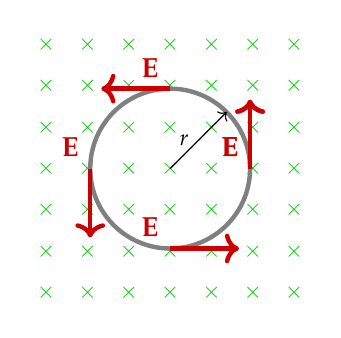
\begin{tikzpicture}[scale=.35]
        \foreach \xx in {-4.5,-3,...,4.5}{
          \foreach \yy in {-4.5,-3,...,4.5}{
            \node at (\xx,\yy) {\footnotesize\textcolor{green!80!black}{$\times$}};
          }
        }
        \draw[gray,ultra thick](0,0) circle(2.9);
        \draw[->,rotate=45](0,0)--(2.9,0) node[midway,left]{\footnotesize $r$};
        \foreach \x in {0,90,...,360} {
          \begin{scope}[rotate=\x]
            \draw[ultra thick,red!80!black,->](2.9,0)--(2.9,2.5)
            node[pos=0,above left]{$\mb{E}$};
          \end{scope}
        }
      \end{tikzpicture}
    \end{center}
    
    \column{.7\textwidth}
    \begin{itemize}
    \item Since \emph{emf} is work per unit charge, that means that there is an
      electric field inside the wire to move the charges.
    \item In this example:
      \begin{itemize}
      \item Magnetic field $\mb{B}$ into the page
      \item The direction of the electric field $\mb{E}$ corresponds to an
        \emph{increase} in magnetic flux
      \end{itemize}
    \end{itemize}
  \end{columns}
\end{frame}


\begin{frame}{Faraday's Law}
  Faraday's law states that the rate of change of magnetic flux produces an
  electromotive force:

  \eq{-.2in}{
    \boxed{
      \mathcal{E}=\oint\mb{E}\cdot d\mb{l}={\color{red}{-}}\frac{d\Phi}{dt}
    }
  }
  
  The negative sign {\textcolor{red}{highlighted in red}} is the result of
  Lenz's law, which is related to the conservation energy
\end{frame}



\begin{frame}{AC Generators}
  A simple AC (alternating current) generator makes use of the fact that a 
  coil rotating against a fixed magnetic field has a changing flux.
  \begin{center}
    \pic{.45}{generator.png}
  \end{center}
  Let's say the permanent magnets produce a uniform magnetic field $B$, and the
  coil between them has $N$ turns, and an area $A$. Now let's say that the coil
  is rotating with an angular frequency $\omega$.
\end{frame}



\begin{frame}{AC Generators}
  \begin{columns}
    \column{.35\textwidth}
    \pic{1}{generator.png}

    \column{.65\textwidth}
    When the coil is turning, the angle between the coil and the magnetic field
    is:
    
    \eq{-.2in}{
      \theta=\omega t+\delta
    } 

    \vspace{-.1in}where $\delta$ is the initial angle. The magnetic flux
    through the coil is given by:
    
    \vspace{-.4in}{\Large
      \begin{align*}
        \Phi&=NBA\cos\theta\\
        &=NBA\cos(\omega t+\delta)
      \end{align*}
    }
    
    \vspace{-.3in}as the coil turns.
  \end{columns}
\end{frame}



\begin{frame}{AC Generators}
  \begin{columns}
    \column{.35\textwidth}
    \pic{1}{generator.png}

    \column{.65\textwidth}  
    The electromotive force \emph{emf} produced is therefore the rate of change
    of the magnetic flux:

    \vspace{-.4in}{\Large
      \begin{align*}
        \mathcal{E} &=-\frac{d\Phi_M}{dt}\\
        &=NBA\omega\sin(\omega t+\delta)
      \end{align*}
    }
  \end{columns}
\end{frame}


\begin{frame}{AC Generators}
  \begin{columns}
    \column{.35\textwidth}
    \pic{1}{generator.png}

    \column{.65\textwidth}
    We commonly write it this way instead:
    
    \eq{-.25in}{\mathcal{E}=\mathcal{E}_{\textrm{max}}\sin(\omega t+\delta)}
    
    \vspace{-.2in}where

    \eq{-.25in}{
      \mathcal{E}_{\textrm{max}}=NBA\omega
    }
  \end{columns}
\end{frame}



\begin{frame}{Motional EMF}
  {What happens when I slide the rod to the right?}
  \begin{columns}
    \column{.45\textwidth}
    \pic{1}{motional-emf-1.png}

    \column{.55\textwidth}
    When sliding the rod to the right with speed $v$, the magnetic flux through
    the loop (and its rate of change) is:

    \vspace{-.4in}{\Large
      \begin{align*}
        \Phi&=BA=B\ell x\\
        \frac{d\Phi}{dt}&=B\ell\frac{dx}{dt}=\boxed{B\ell v=\mathcal{E}}
      \end{align*}
    }
    
    We can use the Lorentz force law on the charges on the rod to find the
    direction of the current $I$.
  \end{columns}
\end{frame}



\begin{frame}{Motional EMF}{What happens when I slide the rod to the right?}
  \begin{columns}
    \column{.25\textwidth}
    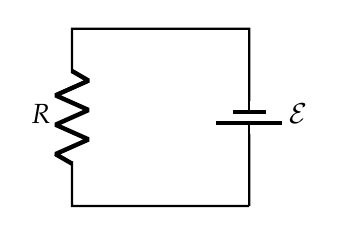
\begin{tikzpicture}[scale=1.5]
      \draw[thick](1.5,0) to[battery1,l_=$\mathcal{E}$] (1.5,1.5)--(0,1.5)
      to[R,l_=$R$] (0,0)--(1.5,0);
    \end{tikzpicture}
    \column{.75\textwidth}
    \begin{itemize}
    \item An equivalent circuit is shown on the left
    \item The amount of current can be found using Ohm's law
    \item Note that the ``motional emf'' produced is spread over the entire
      circuit
    \end{itemize}
  \end{columns}
\end{frame}



\section{Lenz's Law}

\begin{frame}{Lenz's Law}
  Something very interesting happens when the current starts running on the
  wire.
  \begin{center}
    \pic{.35}{motional-emf-2.png}
  \end{center}
  It produces an ``induced magnetic field'' out of the page, in the opposite
  direction as the field that generated the current in the first place.
\end{frame}



\begin{frame}{Lenz's Law}
  \begin{center}
    \fbox{
      \begin{minipage}{.7\textwidth}
        \textbf{LENZ'S LAW}\\
        The induced \emph{emf} and induced current are in such are
        direction as to oppose the change that produces them
      \end{minipage}
    }
  \end{center}

  \vspace{.2in}So basically, the conservation of energy
\end{frame}



\section{Inductance}

\begin{frame}{Back \emph{emf}}
  Consider a very simple circuit consisting of a voltage source and a coil
  \begin{center}
    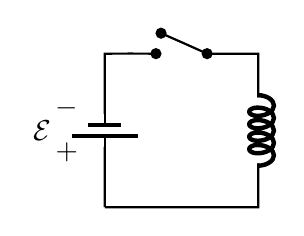
\begin{tikzpicture}[american voltages,scale=1.3]
      \draw[thick](0,0) to[battery1=$\mathcal{E}$] (0,1.5)
      to[short,-*](.5,1.5);
      \draw[thick](.55,1.7) to[short,*-*](1,1.5)--(1.5,1.5)
      to[L] (1.5,0)--(0,0);
    \end{tikzpicture}
  \end{center}
  \begin{itemize}
  \item When the switch is closed and current begins to flow, the coil
    begins to generate a magnetic flux inside
  \item As the current changes (initially increasing with time), it
    self-induces a ``back \emph{emf}'' that opposes the change in current
  \item A current can't jump from zero to some value (or from some value to
    zero) instantaneously
  \end{itemize}
\end{frame}



\begin{frame}{Back \emph{emf}}
  \begin{center}
    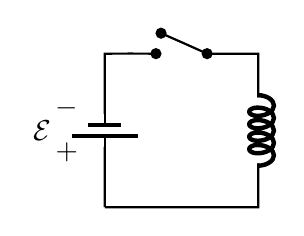
\begin{tikzpicture}[american voltages,scale=1.3]
      \draw[thick](0,0) to[battery1=$\mathcal{E}$] (0,1.5)
      to[short,-*](.5,1.5);
      \draw[thick](.55,1.7) to[short,*-*](1,1.5)--(1.5,1.5)
      to[L] (1.5,0)--(0,0);
    \end{tikzpicture}
  \end{center}
  \begin{itemize}
  \item Breaking the circuit causes the magnetic flux to change very rapidly
  \item The rapid change of $\Phi_M$ creates a large induced back \emph{emf}
    that is proportional to $d\Phi_M/dt$
  \item The back \emph{emf} creates a large voltage drop across the switch
  \item Large voltage across two metal contact produces a very strong electric
    field--strong enough to tear electrons away from air molecules
    (``dielectric breakdown'')
  \item Air conducts electricity in the form of a ``spark''
  \end{itemize}
\end{frame}



\begin{frame}{Self Inductance}
  A solenoid carrying a current generates a magnetic field; its strength given
  by Biot-Savart law (or Amp\`{e}re's law):

  \eq{-.2in}{
    B=\frac{\mu_0NI}{L}
  }

  Since $\mb{B}\propto I$, the magnetic flux through the solenoid (really
  $\Phi=NBA$ where $A$ is the cross-sectional area of the solenoid and $N$ is
  the number of coils) is therefore also proportional to $I$, i.e.

  \eq{-.2in}{
    \boxed{\Phi_M=LI}
  }

  where $L$ is the called the \textbf{self inductance} of the coil.
\end{frame}



\begin{frame}{Self Inductance}
  For a solenoid, we can see that the self inductance is given by:

  \eq{-.2in}{
    \boxed{L=\frac{\Phi_M}{I}=\mu_0 n^2Al}
  }

  where $\mu_0$ is the magnetic permeability of free space, $n$ is the number of
  coil turns per unit length, and $A$ and $l$ are the cross-section and length
  of the solenoid. (i.e. $Al$ is the enclosed volume.)
\end{frame}



\begin{frame}{Self Inductance and Induced EMF}
  If the current changes, the magnetic flux changes as well, therefore inducing
  an electromotive force in the circuit! According Faraday's law:

  \eq{-.2in}{
    \boxed{\mathcal{E}=-\frac{d\Phi_M}{dt}=-L\frac{dI}{dt}}
  }

  The self-induced \emph{emf} is proportional to the rate of change of current
\end{frame}


%\begin{frame}{Mutual Inductance}
%
%\end{frame}



%\section{LR Circuits}
%
%\begin{frame}{Circuits with Inductors}
%  \begin{itemize}
%  \item Coils and solenoids in circuits are known as ``inductors'' and have
%    large self inductance $L$
%  \item Self inductance prevents currents rising and falling instantaneously
%  \item A basic circuit containing a resistor and an inductor is called an
%    \textbf{\emph{LR} circuit}:
%    \begin{center}
%      \begin{tikzpicture}[american voltages,scale=1.2]
%        \draw[thick](0,0) to[battery1=$\mathcal{E}_0$,-*] (0,2)
%        to[short,-*](0.5,2);
%        \draw[thick](0.51,2.3) to[short,*-*](1,2)--(1.5,2) to [R=$R$,-*] (3,2)
%        to [L=$L$,-*] (3,0)--(0,0);
%      \end{tikzpicture}
%    \end{center}
%  \end{itemize}
%\end{frame}
%
%\begin{frame}
%  \frametitle{Analyzing LR Circuits}
%  \begin{columns}
%    \column{.35\textwidth}
%    \begin{tikzpicture}[american voltages,scale=1.2]
%      \draw[thick](0,0) to[battery1=$\mathcal{E}_0$,-*] (0,2)
%      to[short,-*](0.5,2);
%      \draw[thick](0.51,2.3) to[short,*-*](1,2)--(1.5,2) to [R=$R$,-*] (3,2)
%      to [L=$L$,-*] (3,0)--(0,0);
%    \end{tikzpicture}
%
%    \column{.65\textwidth}
%    Applying Kirchkoff's voltage law:
%
%    \eq{-.2in}{\mathcal{E}_0-IR-L\frac{dI}{dt}=0}
%
%    \vspace{-.1in}We follow the same procedure as charging a capacitor to find
%    the time dependent current:
%
%    \eq{-.2in}{I=\frac{\mathcal{E}_0}{R}\left(1-e^{-Rt/L}\right)}
%
%    \vspace{-.15in} The time constant for an $LR$ circuit is
%    
%    \eq{-.2in}{\tau=\frac{L}{R}}
%  \end{columns}
%\end{frame}




\begin{frame}{Magnetic Energy}
  Just as a capacitor stores energy in its electric field, an inductor coil
  carrying a current $I$ stores energy in its magnetic field, given by:

  \eq{-.2in}{
    \boxed{U_M=\frac{1}{2}LI^2}
  }

  We can also define a \textbf{magnetic energy density}:

  \eq{-.2in}{
    \boxed{\eta_M=\frac{B^2}{2\mu_0}}
  }
\end{frame}


%\section{LC Circuit}
%\begin{frame}
%  \frametitle{LC Circuit}
%  The final type of circuit that we will study in AP Physics is the LC
%  circuit. In its simplest form, the circuit has an inductor and capacitor
%  connected in series:
%  \begin{center}
%    \begin{tikzpicture}[american voltages,scale=1.2]
%      \draw[thick](0,0) to[L=$L$] (0,2)--(2,2) to[C=$C$] (2,0)--(0,0);
%    \end{tikzpicture}
%  \end{center}
%  We apply the Kirchkoff's voltage law:
%  
%  \eq{-.2in}{
%    -V_L-V_C=0
%    \quad\rightarrow\quad
%    L\frac{dI}{dt}+\frac{Q}{C}=0
%  }
%\end{frame}
%
%\begin{frame}
%  \frametitle{LC Circuits}
%  Since both terms are continuously differentiable, we can differentiate both
%  sides of the equation, which gives:
%
%  \eq{-.2in}{
%    L\frac{d^2I}{dt^2}+\frac{1}{C}\underbrace{\frac{dQ}{dt}}_I=0
%  }
%
%  In fact, the above equation is one that we have studied many topics ago:
%
%  \eq{-.2in}{
%    \frac{d^2I}{dt^2}+\frac{1}{LC}I=0
%  }
%
%  This is a second-order ordinary differential equation, and the solution is
%  the simple harmonic motion.
%\end{frame}
%
%
%\begin{frame}
%  \frametitle{LC Circuit}
%  The current inside of an LC circuit is given by:
%
%  \eq{-.2in}{
%    I(t)=I_0\sin(\omega t + \varphi)\quad\text{where}\quad
%    \omega=\frac{1}{\sqrt{LC}}
%  }
%\end{frame}
%
\end{document}
